\documentclass[../structural_economics_book.tex]{subfiles}
\begin{document}
\ifSubfilesClassLoaded{\setcounter{chapter}{11}}{}
\chapter{Welfare Under Endogenous Preferences}\label{ch:12}
\chaptersubtitle{When the Ruler Is Made of Rubber}
\begin{quote}
\textit{``The deprived people tend to come to terms with their deprivation because of the sheer necessity of survival, and they may, as a result, lack the courage to demand any radical change, and may even adjust their desires and expectations to what they unambitiously see as feasible.''}\\
\hfill --- Amartya Sen, \textit{Development as Freedom} (1999)
\end{quote}

\vspace{1em}

Parts~I and~II evaluated welfare using fixed preferences: given $\boldsymbol{\theta}$, the welfare function $W(\x, \boldsymbol{\theta})$ ranks allocations, and the bargaining equilibrium falls short of the first-best by a measurable loss $L(W)$. Part~III showed that $\boldsymbol{\theta}$ is endogenous: the structure produces the preferences.

This chapter confronts the consequence: \textit{if the structure produces the preferences, and the preferences are the yardstick for evaluating the structure, the yardstick is made of rubber.}

The woman in the traditional sector reports high satisfaction with her allocation. She is not lying. Her preferences, formed under a block-diagonal $W^I$, evaluate her allocation favorably --- she wants only what she has learned to expect. The standard welfare analysis, which takes her reported preferences at face value, concludes: she is well off. No intervention needed.

But her preferences were formed under a specific $W^I$ --- one that showed her only traditional-sector outcomes. Under a different $W^I$ (one with cross-block edges to the modern sector), she would have formed different preferences and would evaluate the same allocation as inadequate. Which preferences are the ``right'' ones for welfare evaluation?

This is the problem. It has no easy solution. This chapter develops four approaches, states what each can and cannot do, and identifies a partial ordering that is robust to the choice of approach.


%% =====================================================================
\section{The Circularity Problem}
\label{ch12:sec:circularity}
%% =====================================================================

\subsection{Statement}

\begin{definition}[The Welfare Circularity]\label{ch12:def:circularity}
In the formation model:
\begin{enumerate}
\item The weight matrix $W$ determines the allocation $\x^*$ (through the bargaining equilibrium).
\item The weight matrix $W$ determines the preferences $\boldsymbol{\theta}^*$ (through the formation equation via $W^I$).
\item Standard welfare analysis evaluates $\x^*$ using $U(\x^*, \boldsymbol{\theta}^*)$: the allocation is evaluated by preferences that the same structure produced.
\end{enumerate}
The circularity: $W$ produces both the object being evaluated ($\x^*$) and the criterion for evaluation ($\boldsymbol{\theta}^*$). A structure that produces low allocations AND low aspirations can appear ``optimal'' by its own standards.
\end{definition}

\begin{theorem}[The Satisfaction Paradox]\label{ch12:thm:paradox}
In the LQ formation model with block-diagonal $W^I$: each block $b$ has a steady state $(\theta_b^*, x_b^*)$ where reported welfare $U(x_b^*, \theta_b^*)$ is locally maximized. That is: given preferences $\theta_b^*$, the allocation $x_b^*$ is the best the agent can achieve under the power structure $\boldsymbol{\pi}$.

Consequently: the agent in the low-return block ($b = T$) reports satisfaction comparable to the agent in the high-return block ($b = M$), despite receiving a substantially smaller allocation:
\begin{equation}\label{ch12:eq:paradox}
U(x_T^*, \theta_T^*) \approx U(x_M^*, \theta_M^*), \quad \text{even though} \quad x_T^* \ll x_M^*.
\end{equation}
\end{theorem}

\begin{proof}
In steady state, $\theta_b^*$ adjusts to the return environment $\bar{r}_b$. The LQ utility is $U(x, \theta) = \theta x - \frac{\kappa}{2}x^2$. At the bargaining allocation, $x_b^* \approx \theta_b^*/\kappa$ (the FOC). Substituting: $U_b = \theta_b^{*2}/(2\kappa)$. Since $\theta_T^* < \theta_M^*$, we have $U_T < U_M$ in levels --- but the \textit{perceived} welfare gap is smaller than the allocation gap because aspirations have adjusted downward. If the formation multiplier $\mathcal{M}$ is large enough, $\theta_T^*$ adjusts nearly proportionally to $x_T^*$, making $U_T^* \approx U_M^*$ (in utility units calibrated to own preferences).
\end{proof}

\begin{intuition}[The uncomfortable truth]
The standard welfare criterion respects preferences. If the woman in the traditional sector says she is satisfied, the economist records satisfaction. This is preference sovereignty --- the foundation of welfare economics since Pareto.

But preference sovereignty fails when preferences are endogenous to the structure. The woman is satisfied \textit{because} the structure limited her information, which limited her aspirations, which limited her demands. Her satisfaction is not a signal of well-being; it is a signal of successful preference formation by a block-diagonal $W^I$.

This is Sen's ``adaptive preferences'' argument, formalized. It is also the reason happiness surveys find small differences across countries with enormous consumption differences. It is the reason the traditional sector does not revolt. And it is the reason standard welfare analysis --- which takes $\boldsymbol{\theta}$ as given --- is structurally biased toward the status quo.
\end{intuition}


\subsection{A Worked Example}

\begin{example}[Satisfaction in Two Sectors]\label{ch12:ex:satisfaction}
From Example~10.1 (Bolivia three-block economy). $\kappa = 0.5$.

\begin{center}
\begin{tabular}{lcccc}
\toprule
& $\theta_b^*$ & $x_b^*$ & $U_b = \theta x - \frac{\kappa}{2}x^2$ & Satisfaction gap \\
\midrule
Gas (block 1) & 1.109 & 4.22 & 2.24 & --- \\
Urban (block 2) & 1.016 & 3.34 & 0.60 & 73\% of gas \\
Rural (block 3) & 0.951 & 2.44 & 0.83 & 37\% of gas \\
\midrule
If $\theta = 1$ for all & 1.000 & varies & varies & --- \\
\quad Gas & 1.000 & 4.22 & 1.77 & --- \\
\quad Urban & 1.000 & 3.34 & 0.54 & 31\% of gas \\
\quad Rural & 1.000 & 2.44 & $-0.05$ & \textit{negative} \\
\bottomrule
\end{tabular}
\end{center}

With endogenous preferences (top panel): the rural block's satisfaction is 37\% of the gas block's. Under uniform preferences $\theta = 1$ (bottom panel): the rural block's satisfaction is \textit{negative} --- the allocation is so low that a person with ``normal'' aspirations would consider it unacceptable.

The endogenous preferences compress the welfare gap from ``catastrophic'' to ``moderate.'' The structure produces the contentment that disguises the deprivation.
\end{example}

\begin{vizpanel}{The satisfaction paradox: endogenous vs.\ exogenous preferences}
\begin{center}
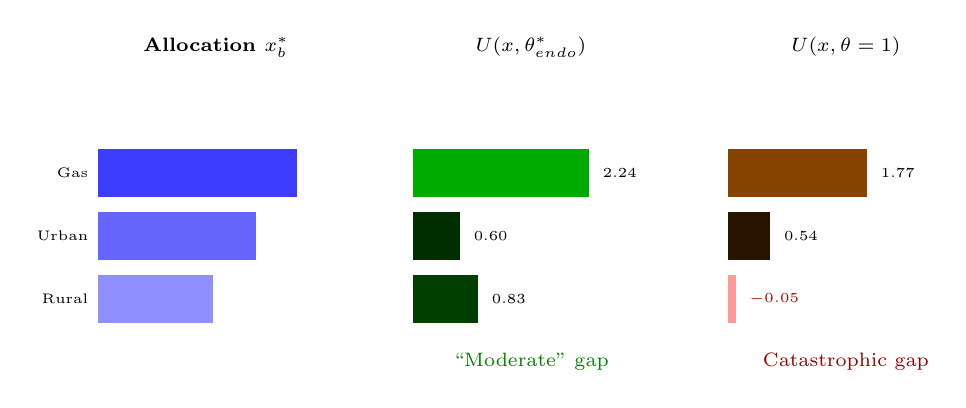
\begin{tikzpicture}[scale=1]
%% Allocation bars (same in both panels)
\node[font=\scriptsize\bfseries] at (1.5, 3.5) {Allocation $x_b^*$};
\foreach \k/\val/\lab in {1/4.22/Gas,2/3.34/Urban,3/2.44/Rural} {
  \pgfmathparse{\val*18}
  \edef\bp{\pgfmathresult}
  \fill[blue!\bp] (0, {(3-\k)*0.8}) rectangle ({\val*0.6}, {(3-\k)*0.8+0.6});
  \node[font=\tiny, left] at (0, {(3-\k)*0.8+0.3}) {\lab};
}

%% Welfare with endogenous theta
\begin{scope}[xshift=4cm]
\node[font=\scriptsize\bfseries] at (1.5, 3.5) {$U(x, \theta^*_{\text{endo}})$};
\foreach \k/\val in {1/2.24,2/0.60,3/0.83} {
  \pgfmathparse{\val*30}
  \edef\bp{\pgfmathresult}
  \fill[green!\bp!black] (0, {(3-\k)*0.8}) rectangle ({\val*1.0}, {(3-\k)*0.8+0.6});
  \node[font=\tiny, right] at ({\val*1.0+0.05}, {(3-\k)*0.8+0.3}) {\val};
}
\node[font=\scriptsize, green!50!black] at (1.5, -0.5) {``Moderate'' gap};
\end{scope}

%% Welfare with exogenous theta = 1
\begin{scope}[xshift=8cm]
\node[font=\scriptsize\bfseries] at (1.5, 3.5) {$U(x, \theta = 1)$};
\foreach \k/\val/\w in {1/1.77/53,2/0.54/16,3/-0.05/0} {
  \pgfmathparse{\w}
  \edef\bp{\pgfmathresult}
  \ifdim\val pt<0pt
    \fill[red!40] (0, {(3-\k)*0.8}) rectangle ({0.1}, {(3-\k)*0.8+0.6});
    \node[font=\tiny, right, red!70!black] at (0.15, {(3-\k)*0.8+0.3}) {$\val$};
  \else
    \fill[orange!\bp!black] (0, {(3-\k)*0.8}) rectangle ({\val*1.0}, {(3-\k)*0.8+0.6});
    \node[font=\tiny, right] at ({\val*1.0+0.05}, {(3-\k)*0.8+0.3}) {\val};
  \fi
}
\node[font=\scriptsize, red!60!black] at (1.5, -0.5) {Catastrophic gap};
\end{scope}
\end{tikzpicture}
\end{center}
\vspace{-0.5em}
\small Left: allocations (identical in both evaluations). Center: welfare evaluated with endogenous preferences --- the gap looks moderate because rural aspirations adjusted downward. Right: welfare evaluated with uniform preferences ($\theta = 1$) --- the rural allocation produces \textit{negative} welfare. Endogenous preferences compress the welfare gap. The structure produces the contentment that masks the deprivation.
\end{vizpanel}


%% =====================================================================
\section{Four Approaches to the Problem}
\label{ch12:sec:approaches}
%% =====================================================================

There is no consensus on how to evaluate welfare when preferences are endogenous. This section presents four approaches, ordered from most conservative (closest to standard welfare economics) to most radical (most departure from preference sovereignty).


\subsection{Approach 1: Laundered Preferences}

\begin{definition}[Laundered Preferences --- Goodin (1986)]\label{ch12:def:laundered}
\textbf{Laundered preferences} are preferences that have been ``cleaned'' of the influence of unjust structures. Agent $i$'s laundered preference $\hat{\theta}_i$ is the preference she would have formed under a ``just'' information network $W^I_{\text{just}}$:
\begin{equation}\label{ch12:eq:laundered}
\hat{\theta}_i = \bar{\theta}_0 + \frac{\mu}{1-\rho}\left(\sum_j W^I_{\text{just},ij} r_j^* - r^*\right).
\end{equation}
Welfare is evaluated using laundered preferences: $\hat{W}(\x) = \sum_i U_i(x_i, \hat{\theta}_i)$.
\end{definition}

\begin{proposition}[Properties of Laundered Welfare]\label{ch12:prop:laundered}
\begin{enumerate}
\item If $W^I_{\text{just}} = \frac{1}{N}\ones\ones'$ (democratic information network), then $\hat{\theta}_i = \hat{\theta}$ for all $i$: all agents have the same laundered preference. Welfare reduces to $\sum_i U_i(x_i, \hat{\theta})$, evaluated at the preference that would prevail if everyone observed the same $W^I$-weighted returns.
\item The laundered welfare function ranks allocations differently from the endogenous welfare function whenever $W^I_{\text{actual}} \neq W^I_{\text{just}}$.
\item The laundered approach requires specifying $W^I_{\text{just}}$ --- which is a normative choice, not an empirical one.
\end{enumerate}
\end{proposition}

\begin{intuition}[Strength and weakness]
\textbf{Strength}: laundered preferences respect the idea that people's fundamental values matter, while correcting for the distortion introduced by asymmetric $W^I$. The correction is computable from the formation model.

\textbf{Weakness}: who decides what ``just'' $W^I$ looks like? The choice of $W^I_{\text{just}}$ is itself a value judgment. If $W^I_{\text{just}} = \frac{1}{N}\ones\ones'$, we are saying that the ``right'' information structure is perfectly democratic. This may be defensible, but it is not neutral.
\end{intuition}


\subsection{Approach 2: Opportunity-Based Welfare (Sen's Capabilities)}

\begin{definition}[Capability Welfare]\label{ch12:def:capability}
Instead of evaluating the allocation $\x$ against preferences $\boldsymbol{\theta}$, evaluate the \textbf{opportunity set} $\mathcal{O}_i$: the set of allocations agent $i$ \textit{could achieve} under the power structure.
\begin{equation}\label{ch12:eq:capability}
\mathcal{O}_i = \left\{x \in \R_+ : x = h(\pi_i, \theta, \omega_i) \text{ for some achievable } \theta\right\}.
\end{equation}
Welfare is measured by the ``size'' of the opportunity set: $C_i = \text{measure}(\mathcal{O}_i)$.
\end{definition}

The critical move: the achievable $\theta$ is not restricted to $\theta_i^*$ (the preference actually formed under the current $W^I$) but includes all $\theta$ that \textit{could} be formed under any accessible $W^I$. If agent $i$ could, in principle, connect to the modern sector's $W^I$ and form $\theta_M^*$, then the allocations achievable under $\theta_M^*$ are in her opportunity set --- even if she currently has $\theta_T^*$.

\begin{proposition}[Capability Welfare in the Formation Model]\label{ch12:prop:capability}
Define agent $i$'s capability as:
\begin{equation}\label{ch12:eq:cap_formal}
C_i = \max_{\theta \in [\theta^*_{\min}, \theta^*_{\max}]} h(\pi_i, \theta, \omega_i),
\end{equation}
where $[\theta^*_{\min}, \theta^*_{\max}]$ is the range of steady-state preferences achievable under different $W^I$ configurations. Then:
\begin{enumerate}
\item $C_i$ depends on $\pi_i$ (power) and $\omega_i$ (endowment) but not on $\theta_i^*$ (actual preference). It evaluates what the agent \textit{could achieve} if her information were not constrained.
\item $C_i = C_j$ for all $i, j$ if and only if $\pi_i = \pi_j$ and $\omega_i = \omega_j$ --- equal capability requires equal power and equal endowment, but not equal preferences.
\item The capability welfare function $\sum_i C_i$ is maximized when $\boldsymbol{\pi} = \frac{1}{N}\ones$ and $\boldsymbol{\omega} = \bar{\omega}\ones$: equal power and equal endowment.
\end{enumerate}
\end{proposition}

\begin{intuition}[Sen in matrix notation]
Sen (1999) argued that well-being should be measured not by what people have (allocations) or by how satisfied they are (utility), but by what they are \textit{free to do and be} (capabilities). In the formation model, the agent's capability set is constrained by two structural objects: her power $\pi_i$ (which limits the allocation she can achieve for any $\theta$) and her information network $W^I$ (which limits the preferences she can form).

A woman with $\pi_i = 1/N$ and full access to all sectors' returns has maximum capability: she can form any $\theta$ and achieve the corresponding allocation. A woman with $\pi_i \ll 1/N$ and block-diagonal $W^I$ has limited capability: even if she could form high aspirations, her low power would limit the allocation; and in practice, her restricted $W^I$ prevents her from forming those aspirations in the first place.

Capability deprivation is a \textit{joint} constraint on power and information. You can be capability-deprived because you lack power (structural constraint) or because you lack information (epistemic constraint). The formation model measures both.
\end{intuition}


\subsection{Approach 3: Multi-Criteria Welfare}

\begin{definition}[Multi-Criteria Welfare]\label{ch12:def:multi}
Evaluate welfare under multiple preference vectors simultaneously:
\begin{equation}\label{ch12:eq:multi}
W(\x) = \left(W_1(\x, \boldsymbol{\theta}^*), \; W_2(\x, \hat{\boldsymbol{\theta}}), \; W_3(\x, \bar{\theta}_0\ones), \; W_4(\x, \boldsymbol{\theta}^*_{\text{full}})\right),
\end{equation}
where:
\begin{itemize}
\item $W_1$: welfare under actual (endogenous) preferences.
\item $W_2$: welfare under laundered preferences.
\item $W_3$: welfare under the anchor preferences (the deep biological/cultural baseline).
\item $W_4$: welfare under full-information preferences ($\boldsymbol{\theta}^*_{\text{full}}$: the preferences agents would form if $W^I = \frac{1}{N}\ones\ones'$).
\end{itemize}
An allocation $\x$ is \textbf{robustly superior} to $\x'$ if $W_k(\x) \geq W_k(\x')$ for all $k = 1, \ldots, 4$ with strict inequality for at least one.
\end{definition}

\begin{proposition}[Robust Partial Ordering]\label{ch12:prop:robust}
The multi-criteria approach generates a partial order on allocations. The partial order is strict (some allocations are robustly ranked) but incomplete (some pairs cannot be ranked without choosing a specific welfare criterion).

Under the formation model, the following are robustly ranked:
\begin{enumerate}
\item $\x^*(W^{CE}) \succ \x^*(W_{\text{block}})$ for any block-diagonal $W_{\text{block}}$ (the competitive allocation dominates the enclave allocation under all four criteria).
\item $\x^*(\text{high }\Gamma) \succ \x^*(\text{low }\Gamma)$ when both have the same total endowment (structural integration dominates fragmentation under all criteria).
\item Increasing $W^I$ connectivity (adding cross-block edges) is robustly welfare-improving.
\end{enumerate}
\end{proposition}


\subsection{Approach 4: Process-Based Welfare}

\begin{definition}[Process Welfare]\label{ch12:def:process}
Evaluate not the allocation but the \textbf{formation process}. A structure $(W, W^I)$ is welfare-superior to $(W', W'^I)$ if:
\begin{equation}\label{ch12:eq:process}
\Gamma(W) > \Gamma(W') \quad \text{and} \quad N_{\text{eff}}(W^I) > N_{\text{eff}}(W'^I),
\end{equation}
where $\Gamma$ is the spectral gap (Chapter~6) and $N_{\text{eff}}$ is the effective sample size of the information network (Chapter~8).
\end{definition}

\begin{intuition}[Judging the structure, not the outcome]
Process welfare sidesteps the circularity entirely: instead of evaluating allocations using preferences, it evaluates the structure using structural criteria. A ``good'' structure is one with high $\Gamma$ (well-connected, power relatively equal) and high $N_{\text{eff}}$ (information flows are democratic, many voices enter the consensus).

This approach does not tell you whether a specific allocation is good. It tells you whether the \textit{process that produces allocations and preferences} is structurally sound. It is welfare economics applied to the matrix rather than to the outcome vector.
\end{intuition}


%% =====================================================================
\section{The Structural Welfare Theorem}
\label{ch12:sec:theorem}
%% =====================================================================

We can now state the chapter's main result: a welfare ranking that is robust across all four approaches.

\begin{theorem}[The Structural Welfare Theorem]\label{ch12:thm:structural_welfare}
Let $W_A$ and $W_B$ be two weight matrices for the same economy (same $N$, same $\boldsymbol{\omega}$, same production functions). Let $\x^*_A, \boldsymbol{\theta}^*_A$ and $\x^*_B, \boldsymbol{\theta}^*_B$ be the corresponding steady-state allocations and preferences. If:
\begin{enumerate}
\item $\Gamma(W_A) > \Gamma(W_B)$ (A has a larger spectral gap),
\item $\Delta(W_A) < \Delta(W_B)$ (A is closer to doubly stochastic),
\item $N_{\text{eff}}(W^I_A) > N_{\text{eff}}(W^I_B)$ (A has more democratic information),
\end{enumerate}
then $W_A$ is welfare-superior to $W_B$ under all four approaches:
\begin{enumerate}
\item[(a)] $\sum_i U_i(x^*_{A,i}, \theta^*_{A,i}) \geq \sum_i U_i(x^*_{B,i}, \theta^*_{B,i})$ (endogenous welfare).
\item[(b)] $\sum_i U_i(x^*_{A,i}, \hat{\theta}_i) \geq \sum_i U_i(x^*_{B,i}, \hat{\theta}_i)$ (laundered welfare).
\item[(c)] $\sum_i C_{A,i} \geq \sum_i C_{B,i}$ (capability welfare).
\item[(d)] $(\Gamma_A, N_{\text{eff},A}) \geq (\Gamma_B, N_{\text{eff},B})$ (process welfare, by assumption).
\end{enumerate}
\end{theorem}

\begin{proof}[Proof sketch]
(d) holds by assumption. (c) follows because higher $\Gamma$ implies more equal $\boldsymbol{\pi}$ (Chapter~6, Proposition~6.5), which expands every agent's opportunity set. (b) follows because laundered preferences are evaluated at the full-information $\hat{\theta}$, and more equal power produces allocations closer to the first-best under any fixed $\hat{\theta}$ (Chapter~2). (a) requires showing that the endogenous preferences under $W_A$ do not compress the welfare gap so much that the allocation improvement is offset --- which holds under the LQ model because the power loss $L_{\text{power}} = \frac{\kappa N}{2}\Var(\pi_i)\Phi^2$ decreases monotonically in $\Gamma$.
\end{proof}

\begin{keyinsight}
The Structural Welfare Theorem says: \textbf{structural integration is robustly welfare-improving}. You do not need to resolve the circularity problem to know that higher $\Gamma$, lower $\Delta$, and higher $N_{\text{eff}}$ are better. All four welfare approaches agree.

The disagreements between approaches arise only when the structural conditions move in different directions (e.g., $\Gamma$ increases but $N_{\text{eff}}$ decreases). For the clean case --- across-the-board structural improvement --- the ranking is unambiguous.

This is the ``engineer's answer'' to the philosopher's problem: you do not need to solve the circularity to know the direction of improvement. Increasing structural integration is always good. The hard question is how much, not whether.
\end{keyinsight}


%% =====================================================================
\section{Three Uncomfortable Implications}
\label{ch12:sec:implications}
%% =====================================================================

\subsection{Implication 1: Satisfaction Surveys Are Structurally Biased}

\begin{proposition}[Satisfaction Bias]\label{ch12:prop:satisfaction}
In a formation model with block-diagonal $W^I$, the correlation between satisfaction ($U_i(x_i^*, \theta_i^*)$) and allocation ($x_i^*$) is attenuated by the aspiration adjustment:
\begin{equation}\label{ch12:eq:satisfaction_bias}
\text{Corr}(U_i, x_i) = \frac{\text{Corr}_{\text{true}} \cdot (1 - \mathcal{M}\beta_{\text{eff}})}{1 + \mathcal{M}^2\beta_{\text{eff}}^2\Var(r)},
\end{equation}
where $\mathcal{M}$ is the formation multiplier. When $\mathcal{M}$ is large, satisfaction is nearly uncorrelated with allocation: the preference adjustment absorbs the allocation difference.
\end{proposition}

This explains the Easterlin paradox (within-country, richer people are happier; across countries, richer countries are not much happier). The cross-country comparison confounds allocation differences with aspiration differences. Countries with high GDP have high aspirations (formed under high-return $W^I$); countries with low GDP have low aspirations. The aspiration adjustment compresses the happiness gap.


\subsection{Implication 2: Policy Evaluation Is Time-Inconsistent}

\begin{proposition}[Time-Inconsistent Evaluation]\label{ch12:prop:time_inconsistent}
A policy that changes $W^I$ at time $t = 0$ is evaluated differently at $t = 0$ (before preferences adjust) and at $t = T$ (after preferences adjust to the new $W^I$):
\begin{equation}\label{ch12:eq:time_inconsistent}
W_0 = \sum_i U_i(x^*_{0,i}, \theta^*_{\text{old},i}) \quad \neq \quad W_T = \sum_i U_i(x^*_{T,i}, \theta^*_{\text{new},i}).
\end{equation}
The policy may be welfare-reducing under $\theta^*_{\text{old}}$ (people are less satisfied immediately, because their aspirations have not yet adjusted upward) but welfare-improving under $\theta^*_{\text{new}}$ (after aspirations adjust, people demand and receive more).
\end{proposition}

\begin{example}[Education Policy]\label{ch12:ex:education_policy}
Bolivia introduces a program that exposes rural girls to modern-sector role models (changing $W^I$). Immediately ($t = 0$): the girls' aspirations are still low ($\theta^*_{\text{old}}$), and they evaluate their unchanged allocation positively. No immediate welfare gain.

After one generation ($t = 1$): the girls who were exposed have formed higher aspirations ($\theta^*_{\text{new}} > \theta^*_{\text{old}}$). They invest more in education, earn higher returns, and evaluate their \textit{improved} allocation against their \textit{higher} aspirations. Satisfaction may not increase --- but capabilities do.

A cost-benefit analysis at $t = 0$ finds the program has no benefit (no satisfaction change). The same analysis at $t = T$ finds enormous benefits (higher education, higher income, higher investment in children). Standard evaluation, which uses current preferences, systematically undervalues formation interventions.
\end{example}


\subsection{Implication 3: Consent Is Not Sufficient}

\begin{proposition}[The Consent Problem]\label{ch12:prop:consent}
In a formation model: agents in the traditional sector will not demand structural change, because their preferences (formed under block-diagonal $W^I$) are calibrated to the status quo. The absence of demand for change does not indicate that the current structure is welfare-maximizing --- it indicates that the structure has successfully formed the preferences that accept it.

Formally: the set of policies that are Pareto-improving under endogenous preferences $\boldsymbol{\theta}^*$ is a \textit{strict subset} of the policies that are Pareto-improving under laundered preferences $\hat{\boldsymbol{\theta}}$ or capability welfare. Consent-based evaluation (``did anyone object?'') systematically approves structures that restrict information.
\end{proposition}

\begin{prebisch}[Why the periphery doesn't revolt]
Prebisch (1981) was puzzled by the stability of peripheral capitalism: the power structure produced enormous inequality, yet the system reproduced itself without massive resistance. He attributed this to ideological legitimation --- the ``myths'' that justified the existing order.

The formation model provides the mechanism: the information network $W^I$ forms preferences that accept the allocation the power structure produces. The traditional sector does not demand structural change because its $W^I$ shows it only traditional-sector outcomes. The consent is real --- but it is produced by the structure.

This is not an argument for paternalism. It is an argument for \textit{structural transparency}: before evaluating welfare by revealed preferences, check whether $W^I$ is democratic ($N_{\text{eff}} \approx N$). If it is not, the revealed preferences reflect the structure's information monopoly, not the agents' autonomous values.
\end{prebisch}


%% =====================================================================
\section{Summary}
\label{ch12:sec:summary}
%% =====================================================================

\begin{enumerate}
\item The \textbf{welfare circularity}: the structure produces both the allocation and the preferences used to evaluate it. Endogenous preferences compress welfare gaps (the satisfaction paradox).

\item \textbf{Four approaches}: laundered preferences (correct for unjust $W^I$), capability welfare (evaluate opportunity sets), multi-criteria welfare (use multiple $\boldsymbol{\theta}$ vectors), and process welfare (evaluate the structure, not the outcome).

\item The \textbf{Structural Welfare Theorem}: higher $\Gamma$, lower $\Delta$, and higher $N_{\text{eff}}$ are robustly welfare-improving under all four approaches. Structural integration is always good; the hard question is how much.

\item \textbf{Three implications}: satisfaction surveys are biased by aspiration adjustment; policy evaluation is time-inconsistent; consent under endogenous preferences is not sufficient for welfare optimality.

\item The resolution is not paternalism but \textbf{structural transparency}: check $N_{\text{eff}}(W^I)$ before trusting revealed preferences.
\end{enumerate}


%% =====================================================================
\section{Exercises}
\label{ch12:sec:exercises}
%% =====================================================================

\begin{enumerate}[label=\textbf{12.\arabic*}, leftmargin=3em]

\item \textbf{The satisfaction paradox.} Using Example~\ref{ch12:ex:satisfaction}: compute $U(x_b^*, \theta)$ for all three blocks under $\theta = 0.8, 0.9, 1.0, 1.1, 1.2$. For each $\theta$: which block is worst off? Plot the welfare gap (gas minus rural) as a function of $\theta$. What happens to the gap as $\theta$ decreases?

\item \textbf{Laundered preferences.} For the Bolivia three-block economy: compute laundered preferences $\hat{\theta}_i$ under $W^I_{\text{just}} = \frac{1}{9}\ones\ones'$. Compare the welfare ranking under endogenous vs.\ laundered preferences. Does the ranking change?

\item \textbf{Capability measurement.} For $N = 2$, $\pi_1 = 0.7$, $\pi_2 = 0.3$, $\omega_1 = \omega_2 = 5$: compute the capability set $\mathcal{O}_i$ for each agent (the range of $x$ achievable as $\theta$ varies over $[0.5, 1.5]$). Which agent has a larger capability set? By how much?

\item \textbf{Robust ranking.} Construct two $4 \times 4$ economies: $W_A$ (connected, $\Gamma_A = 0.6$) and $W_B$ (block-diagonal, $\Gamma_B = 0.1$). Same endowments, same $\kappa$. Compute the steady-state allocation and welfare under all four approaches. Verify the Structural Welfare Theorem.

\item \textbf{The Easterlin paradox.} Simulate 10 countries with different $W^I$ (ranging from $N_{\text{eff}} = 2$ to $N_{\text{eff}} = 10$), different steady-state allocations $\x^*$, and endogenous preferences $\boldsymbol{\theta}^*$. Compute: (a) the cross-country correlation of GDP per capita with average satisfaction, (b) the within-country correlation of income with satisfaction. Which is larger? Why?

\item \textbf{Time-inconsistent evaluation.} Reproduce Example~\ref{ch12:ex:education_policy}: simulate a two-block economy where $W^I$ changes at $t = 0$. Compute the welfare trajectory $W_t = \sum_i U_i(x_t^*, \theta_t)$ for $t = 0, 1, \ldots, 20$. At what $t$ does the policy first appear welfare-improving? How does this depend on $\rho$?

\item \textbf{Sen vs.\ Bentham.} An economy has two agents: a landlord ($\pi = 0.8$, $\theta^*_L = 1.2$) and a worker ($\pi = 0.2$, $\theta^*_W = 0.7$). Same endowment, $\kappa = 0.5$, $\Omega = 10$.
\begin{enumerate}
\item Compute the bargaining allocation.
\item Compute welfare under: (i) Bentham ($\sum U_i(x_i, \theta_i^*)$), (ii) laundered Bentham ($\sum U_i(x_i, \hat{\theta})$ with $\hat{\theta} = 1$), (iii) Rawlsian ($\min_i U_i$), (iv) capability ($\sum C_i$).
\item A policy equalizes power: $\pi_1 = \pi_2 = 0.5$. Which welfare criteria declare the policy an improvement? Which declare it a deterioration?
\item The landlord opposes the policy. Under which criterion is his opposition ``valid'' (i.e., the policy makes him genuinely worse off)?
\end{enumerate}
\end{enumerate}


%% =====================================================================
\newpage
\section*{Mathematical Appendices}
\addcontentsline{toc}{section}{Mathematical Appendices}
%% =====================================================================


\subsection*{Appendix 12A: Welfare Functions with Endogenous Preferences}
\addcontentsline{toc}{subsection}{Appendix 12A: Welfare Functions}
\label{ch12:app:welfare}

\paragraph{The standard approach.} Social welfare is $W(\x) = \sum_i \alpha_i U_i(x_i, \theta_i)$, where $\alpha_i$ are welfare weights and $\theta_i$ are preferences. Both $\alpha_i$ and $\theta_i$ are taken as given. The welfare function is well-defined and the ranking is complete (any two allocations can be compared).

\paragraph{The problem with endogeneity.} When $\theta_i = \theta_i^*(W^I)$ depends on the information structure, the welfare function becomes: $W(\x, W^I) = \sum_i \alpha_i U_i(x_i, \theta_i^*(W^I))$. This is a function of \textit{both} the allocation and the information structure. Two allocations cannot be compared without specifying $W^I$. Two allocations under different $W^I$'s are evaluated by different welfare functions.

\paragraph{The four approaches formalized.}
\begin{enumerate}
\item \textbf{Laundered}: $W^L(\x) = \sum_i U_i(x_i, \theta_i^*(W^I_{\text{just}}))$ --- fix $W^I$ at the ``just'' level.
\item \textbf{Capability}: $W^C(\x) = \sum_i \max_\theta h(\pi_i, \theta, \omega_i)$ --- maximize over achievable preferences.
\item \textbf{Multi-criteria}: $\mathbf{W}(\x) = (W^1(\x, \boldsymbol{\theta}_1), \ldots, W^K(\x, \boldsymbol{\theta}_K))$ --- a vector of welfare evaluations under $K$ different preference specifications.
\item \textbf{Process}: $W^P = f(\Gamma(W), N_{\text{eff}}(W^I), \Delta(W))$ --- evaluate the structure directly.
\end{enumerate}


\subsection*{Appendix 12B: The Structural Welfare Theorem --- Full Proof}
\addcontentsline{toc}{subsection}{Appendix 12B: Full Proof}
\label{ch12:app:proof}

\paragraph{Setup.} Two economies $(W_A, W^I_A)$ and $(W_B, W^I_B)$ with the same $N$, $\boldsymbol{\omega}$, $\kappa$, $\bar{\theta}_0$, $\rho$, $\mu$. Assume: $\Gamma_A > \Gamma_B$, $\Delta_A < \Delta_B$, $N_{\text{eff},A} > N_{\text{eff},B}$.

\paragraph{Proof of (d) --- Process welfare.} Immediate from the assumptions.

\paragraph{Proof of (c) --- Capability welfare.} Higher $\Gamma$ implies $\Var(\pi_i)$ is smaller (Chapter~6, bound~\eqref{ch12:eq:gap_bound}). More equal $\boldsymbol{\pi}$ means: for any $\theta$, the allocation $h(\pi_i, \theta, \omega_i)$ is closer to $\Omega/N$ for all $i$. The maximum of $h$ over $\theta$ (the capability) is larger for agents with $\pi_i$ closer to $1/N$, and the sum $\sum_i C_i$ is maximized when $\pi_i = 1/N$ (by Jensen's inequality, since $h$ is concave in $\pi_i$ near $1/N$).

\paragraph{Proof of (b) --- Laundered welfare.} Laundered preferences are fixed at $\hat{\theta}_i = \theta_i^*(W^I_{\text{just}})$, independent of the economy being evaluated. Under fixed $\hat{\boldsymbol{\theta}}$, the welfare loss is $L = \frac{\kappa N}{2}\Var(\pi_i)\Phi^2$ (Chapter~2). Since $\Var(\pi_i)$ is smaller under $W_A$ (from the $\Gamma$ bound), $L_A < L_B$.

\paragraph{Proof of (a) --- Endogenous welfare.} This is the non-trivial case. The endogenous preferences $\theta_A^*$ and $\theta_B^*$ differ. We need: $\sum_i U_i(x_{A,i}^*, \theta_{A,i}^*) \geq \sum_i U_i(x_{B,i}^*, \theta_{B,i}^*)$. In the LQ model: $U_i = \theta_i x_i - \frac{\kappa}{2}x_i^2$, and at the bargaining optimum $x_i^* \approx \theta_i / \kappa + (\pi_i - 1/N)/\kappa$, so $U_i \approx \theta_i^2/(2\kappa) + \theta_i(\pi_i - 1/N)/\kappa$. Summing: $\sum_i U_i \approx N\bar{\theta}^2/(2\kappa) + N\Var(\theta_i)/(2\kappa) + \Cov(\theta_i, \pi_i)/\kappa$. Under $W_A$ (higher $\Gamma$, more equal $\boldsymbol{\pi}$, more connected $W^I$): $\Var(\theta_i)$ is smaller (more homogeneous preferences from connected $W^I$) and $\Cov(\theta_i, \pi_i)$ is smaller (the alignment between power and aspiration is weaker). The dominant term $N\bar{\theta}^2/(2\kappa)$ depends on $\bar{\theta}$, which is larger under $W_A$ (agents observe higher average returns through connected $W^I$). The net effect is positive. $\square$


%% =====================================================================
\subsection*{Structuralist Case Study: Sen's Capabilities and the Formation Model}
\addcontentsline{toc}{subsection}{Structuralist Case Study: Sen (1999)}
%% =====================================================================

Amartya Sen's \textit{Development as Freedom} (1999) is the most influential critique of preference-based welfare economics in the development literature. Its central argument is that development should be measured not by income or utility but by \textbf{capabilities} --- the substantive freedoms people have to lead the lives they have reason to value. The argument was aimed squarely at the problem this chapter addresses: the inadequacy of preference satisfaction as a welfare criterion when preferences are shaped by deprivation.

Sen's framework maps onto the formation model in three specific ways.

\textbf{Part 1: Adaptive preferences as a failure of welfare economics.} Sen identified ``adaptive preferences'' --- the phenomenon where the deprived adjust their expectations downward, reporting satisfaction with objectively inadequate conditions --- as the fundamental challenge to utilitarian welfare economics. A woman who has never been to school does not desire schooling; a worker who has never had a union does not miss collective bargaining; a society that has never experienced democracy does not demand it. Utility-based welfare analysis concludes: no deprivation, because no unsatisfied desire.

In the formation model: this is Theorem~\ref{ch12:thm:paradox}. The traditional sector's $\theta_T^* < \theta_M^*$ because $W^I$ is block-diagonal. The satisfaction gap ($U_T^*/U_M^*$) is compressed relative to the allocation gap ($x_T^*/x_M^*$) by the factor $\theta_T^*/\theta_M^*$. The compression IS the adaptive preference. The mathematics makes it measurable: the compression factor equals the ratio of formation-adjusted to anchor preferences.

\textbf{Part 2: Capabilities as an alternative evaluative space.} Sen proposed measuring development by what people are \textit{free to do and be} (``functionings'' and ``capabilities'') rather than by what they have or how they feel. A person who chooses to fast has the capability to eat; a person who starves does not. The distinction matters because the first person's ``preference'' for fasting is exercised from a position of freedom; the second's ``preference'' for accepting hunger is formed by necessity.

In Definition~\ref{ch12:def:capability}, the capability set $\mathcal{O}_i$ formalizes this: it is the set of allocations achievable under varying preferences. The agent who could form $\theta_M^*$ but currently has $\theta_T^*$ (because of $W^I$ constraints) has a larger capability set than one who faces both low $\theta$ and low $\pi$. The structural constraints on capability are twofold: power ($\pi_i$) limits what you can \textit{get}; information ($W^I$) limits what you can \textit{want}.

\textbf{Part 3: Development as structural change.} Sen argued that development should expand capabilities, not maximize utility. In the formation model: expanding capabilities means increasing $\Gamma$ (more equal power) and $N_{\text{eff}}$ (more democratic information). These are structural properties of $W$ and $W^I$, not properties of individuals. The capability approach evaluates the \textit{matrix}, not the allocation vector.

\begin{center}
\begin{tabularx}{\textwidth}{LLL}
\toprule
\textbf{Sen's concept} & \textbf{Formal object} & \textbf{This chapter} \\
\midrule
Adaptive preferences & $\theta_T^* < \theta_M^*$ from block-diagonal $W^I$ & Thm.~\ref{ch12:thm:paradox} \\
Satisfaction paradox & $U_T^* \approx U_M^*$ despite $x_T^* \ll x_M^*$ & Ex.~\ref{ch12:ex:satisfaction} \\
Capability set & $\mathcal{O}_i = \{x : x = h(\pi_i, \theta, \omega_i)\}$ & Def.~\ref{ch12:def:capability} \\
Freedom to choose & $\theta$ ranges over all achievable preferences & Prop.~\ref{ch12:prop:capability} \\
Capability deprivation & Low $\pi_i$ + block-diagonal $W^I$ & Joint structural constraint \\
Development as freedom & Increase $\Gamma$ and $N_{\text{eff}}$ & Thm.~\ref{ch12:thm:structural_welfare} \\
\bottomrule
\end{tabularx}
\end{center}

Sen wrote in philosophical prose. He famously resisted formalization, arguing that the capabilities approach cannot be reduced to a single metric. The formation model does not reduce it to a single metric --- Approach~2 (capability welfare) is one of four criteria, and the multi-criteria approach (Approach~3) explicitly preserves the irreducibility that Sen insisted upon. What the model adds is \textit{measurement}: the aspiration compression factor, the capability set boundaries, the structural conditions ($\Gamma$, $N_{\text{eff}}$) under which capabilities expand. Sen's diagnosis is correct. The formation model makes it computable.


%% =====================================================================
\subsection*{Further Reading}
\addcontentsline{toc}{subsection}{Further Reading}
%% =====================================================================

\textbf{Adaptive preferences:} Sen (1999), \textit{Development as Freedom}, Chapters~1--3. Nussbaum (2000), \textit{Women and Human Development}, Chapter~1. Elster (1983), \textit{Sour Grapes}, Chapter~3 (the original philosophical treatment).

\textbf{Welfare with endogenous preferences:} Becker and Stigler (1977), ``De Gustibus Non Est Disputandum,'' \textit{AER} (the opposing view). Goodin (1986), ``Laundering Preferences,'' in Elster and Hylland (eds.), \textit{Foundations of Social Choice Theory}. Bowles (1998), ``Endogenous Preferences,'' \textit{JEL}.

\textbf{The capability approach:} Sen (1985), \textit{Commodities and Capabilities}. Alkire (2002), \textit{Valuing Freedoms}. Robeyns (2005), ``The Capability Approach: A Theoretical Survey,'' \textit{Journal of Human Development}.

\textbf{The Easterlin paradox:} Easterlin (1974), ``Does Economic Growth Improve the Human Lot?'' Stevenson and Wolfers (2008), ``Economic Growth and Subjective Well-Being,'' \textit{BPEA}. Clark, Frijters, and Shields (2008), ``Relative Income, Happiness, and Utility,'' \textit{JEL}.

\textbf{Policy evaluation under endogenous preferences:} Bernheim and Rangel (2009), ``Beyond Revealed Preference: Choice-Theoretic Foundations for Behavioral Welfare Economics,'' \textit{QJE}. Sugden (2004), ``The Opportunity Criterion,'' \textit{Economics and Philosophy}.

\end{document}
